%!TEX root = <main.tex>
\appendix

\section{Interactive Mode Execution}

\begin{figure}[t]
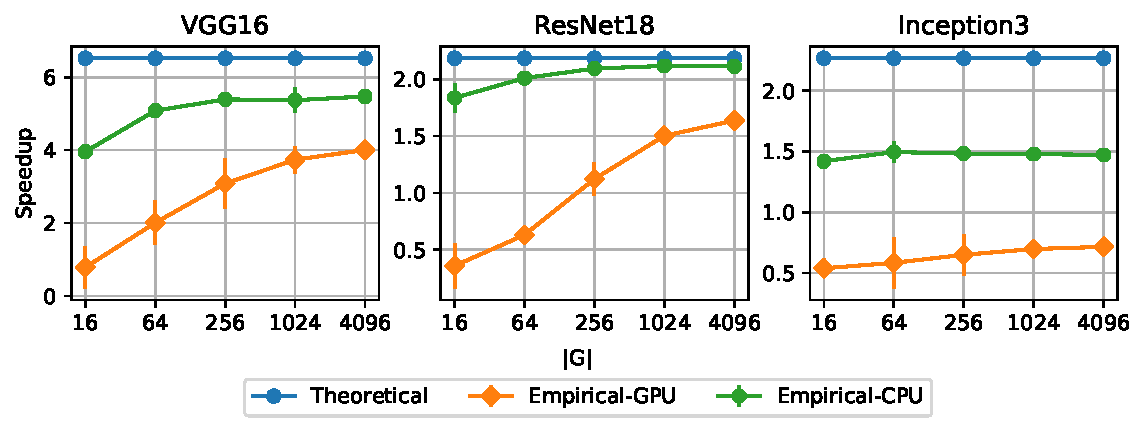
\includegraphics[width=\columnwidth]{images/interactive_experiment.pdf}
\vspace{-8mm}
\caption{Interactive mode execution of incremental inference with $G$s of different sizes}
\label{fig:interactive_experiment}
\end{figure}

We evaluate interactive-mode incremental inference execution (no approximate inference optimizations) with $G$s of different sizes.
Similar to non-interactive mode experiments presented in Section 5, all experiments are run in batched mode with a batch size of 16 for CPU based experiments and a batch size 128 for GPU based experiments.
If the size of $G$ (formally $|G|$) or the remainder of $G$ is smaller than the batch size, that value is used as the batch size (e.g. $|G| = 16$ results in a batch size of 16).
Figure \ref{fig:interactive_experiment} presents the final results.

\section{GPU-Optimized Kernel Implementation}

\begin{figure}[t]
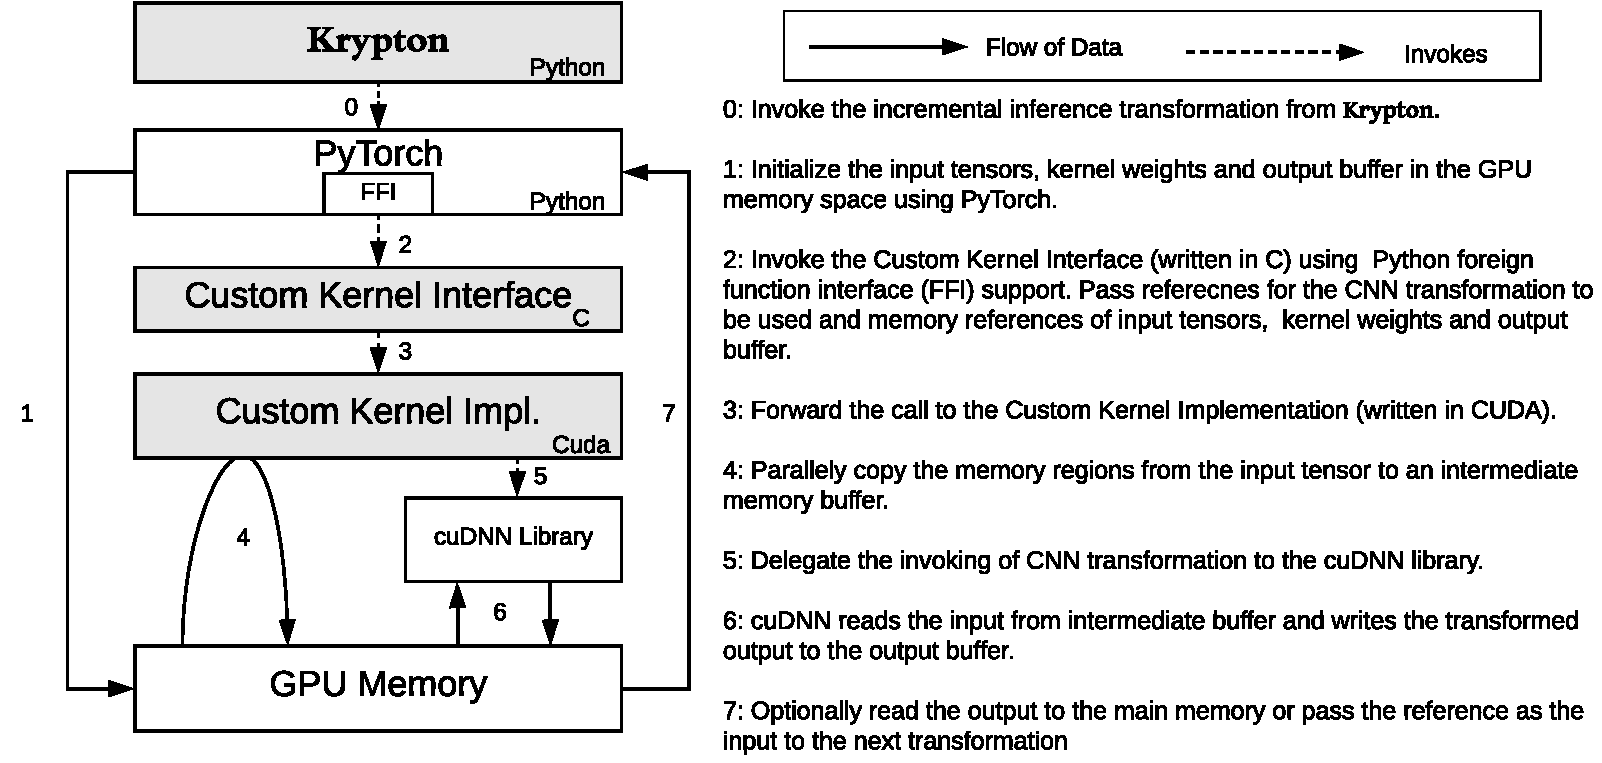
\includegraphics[width=\columnwidth]{images/gpu_kernel_impl.pdf}
\vspace{-8mm}
\caption{Custom GPU Kernel integration architecture}
\label{fig:custom_kernel_integration}
\end{figure}

We extend PyTorch by adding a custom GPU kernel which optimizes the input preparation for \textit{incremental inference} by invoking parallel memory copy operations.
This custom kernel is integrated to PyTorch using Python foreign function interface (FFI).
Python FFI integrates with the Custom Kernel Interface layer which intern invokes the Custom Kernel Implementation.
The high-level architecture of the Custom Kernel integration is shown in Figure~\ref{fig:custom_kernel_integration}


\section{Special Cases for Incremental Inference}

\begin{figure}[t]
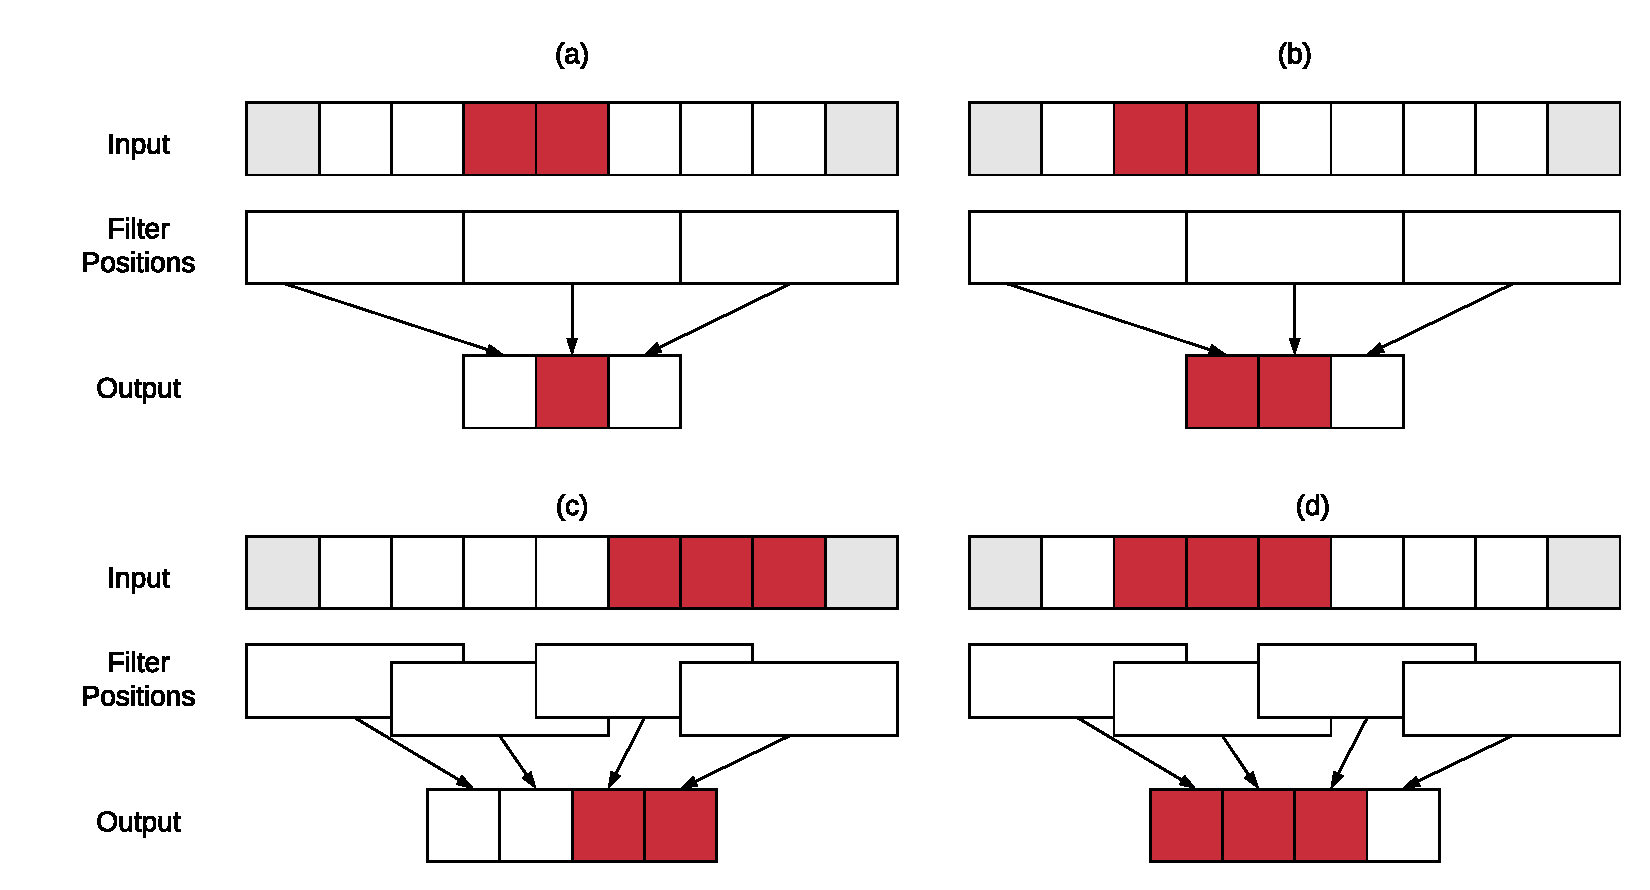
\includegraphics[width=\columnwidth]{images/less_one_example}
\vspace{-6mm}
\caption{1-D illustration of special cases for which actual output size will be smaller than the value given by Equation~(\ref{eqn:xcoordinate}). (a) and (b) show cases with filter stride equal to filter size. (c) and (d) show with input update patch being placed at the edge of the input.}
\vspace{-4mm}
\label{fig:less_one_example}
\end{figure}

There are special cases under which the actual output update patch size can be smaller than the values given by Section~\ref{sec:inc_computation}. Consider the simplified 1-D case shown in Figure~\ref{fig:less_one_example}(a), wherein the stride\footnote{Note that stride is typically less than or equal to filter size.} (3) is the same as filter size (3). In this cases, the size of the output update patch is 1 less than the value given by Equation~(\ref{eqn:patchwidth}). But this is not the case in Figure~\ref{fig:less_one_example}(b), which has the same input update patch size but placed at a different location.
% This issue arises only when the stride value is same as the filter size.
Another case arises when the input update patch is placed at the edge of the input, as shown in Figure~\ref{fig:less_one_example}(c). In this case, it is impossible for the filter to move freely through all positions, since it hits the input boundary, compared against having the input update patch on the middle of the input, as shown in Figure \ref{fig:less_one_example}(c). In \system, we do not treat theses cases separately but rather use the values given by Equation~(\ref{eqn:patchwidth}) for the width dimension (similarly height dimension), since they act as upper bounds. In case of a smaller output update patch, \system~ just reads off and updates slightly bigger patches to preserve uniformity. This also requires updating the start coordinates of the patches, as shown in Equation~(\ref{eqn:width_subtract}). This sort of uniform treatment is required for performing batched inference operations, which gives significant speedups out of the box compared to per-image inference.

\vspace{-4mm}
\begin{align}
\begin{split}
\label{eqn:width_subtract}
&\text{If~} x^\mathcal{O}_\mathcal{P} + ~W^\mathcal{O}_\mathcal{P} > W_{\mathcal{O}}:\\
&x^\mathcal{O}_\mathcal{P} ~ =  W_{\mathcal{O}} - W^\mathcal{O}_\mathcal{P}; 
x^\mathcal{I}_\mathcal{P} ~ = W_{\mathcal{I}} - W^\mathcal{I}_\mathcal{P}; 
x^\mathcal{R}_\mathcal{P} ~ = W_{\mathcal{I}} - W^\mathcal{R}_\mathcal{P}
\end{split}
\end{align}





\section{Effective Projective Field Size (1-D Scenario)}

We formalize the effective projective field growth for the one dimensional scenario with $n$ convolution layers (assuming certain conditions).

The input is $u(t)$ where
\begin{align}
	u(t) = 
	\begin{cases}
		1, & t = 0\\
		0, & t \neq 0 
	\end{cases}
\end{align}
and $t = 0, 1, -1, 2, -2, ...$ indexes the input pixels.

Each layer has the \textbf{same kernel} $v(t)$ of size $k$. The kernel signal can be formally defined as
\begin{align}
	v(t) = \sum_{m=0}^{k-1} w(m)\delta(t-m)
\end{align}
where $w(m)$ is the weight for the $m$th pixel in the kernel.
Without loosing generality, we can assume the weights are normalized, i.e. $\sum_{m}w(w)=1$. The output signal of the $n$th layer $o(t)$ is simply $o = u * v * ... * v$, convolving $u$ with $n$ such $v$\'s.
To compute the convolution, we can use the Discrete Time Fourier Transform to convert the signals into the Fourier domain, and obtain
\begin{align}
\begin{split}
	U(\omega) =&~ \sum_{t=-\infty}^{\infty} u(t)e^{-j\omega t} = 1, ~V(\omega) \\=&~ \sum_{t=-\infty}^{\infty} v(t)e^{-j\omega t} = \sum_{m=0}^{k-1} w(m)e^{-j\omega t}
\end{split}
\end{align}

Applying the convolution theorem, we have the Fourier transform of $o$ is
\begin{align}
\begin{split}
	\mathcal{F}(o) =&~ \mathcal{F}(u*v*...*v)(\omega) = U(\omega) . V(\omega)^n \\=&~ \Bigg(\sum_{m=0}^{k-1}w(m)e^{-j\omega t}\Bigg)^n
\end{split}
\end{align}

With inverse Fourier transform
\begin{align}
	o(t) = \frac{1}{2\pi}\int_{-\pi}^{\pi}\Big(\sum_{m=0}^{k-1}w(m)e^{-j\omega t}\Big)^ne^{j\omega t} d\omega
\end{align}

The space domain signal $o(t)$ is given by the coefficients of $e^{-j\omega t}$.
These coefficients turn out to be well studied in the combinatorics literature \cite{eger2013restricted}.
It can be shown that if $\mathbf{\sum_{m}w(m) = 1}$  and $\mathbf{w(m) \geq 0 ~\forall~ m}$ , then
\begin{align}
\begin{split}
	o(t) =&~ p(S_n=t)\\ 
	\text{where}~ S_n =&~ \sum_{i=1}^{n} X_i ~\text{and}~p(X_i=m) = w(m)
\end{split}
\end{align}

From the central limit theorem, as $n \rightarrow~\infty$, $\sqrt{n}(\frac{1}{n}S_n - \mathop{\mathbb{E}}[X]) \sim \mathcal{N}(0, Var[X])$ and $S_n \sim \mathcal{N}(n\mathop{\mathbb{E}}[X]), nVar[X])$.
As $o(t) = p(S_n=t)$, $o(t)$ also has a Gaussian shape with
\begin{align}
	\mathop{\mathbb{E}}[S_n] =&~ n\sum_{m=0}^{k-1}mw(m)\\
	Var[S_n] =&~ n \Bigg(\sum_{m=0}^{k-1}m^2w(m) - \Big(\sum_{m=0}^{k-1}mw(m)\Big)^2 \Bigg)
\end{align}

This indicates that $o(t)$ decays from the center of the projective field squared exponentially according to the Gaussian distribution.
As the rate of decay is related to the variance of the Gaussian and assuming the size of the effective projective field is one standard deviation, the size can be expressed as
\begin{align}
	\sqrt{Var[S_n]} = \sqrt{nVar[X_i]} = O(\sqrt{n})
\end{align}

On the other hand stacking more convolution layers would grow the theoretical projective field linearly. But the effective projective field size is shrinking at a rate of $O(1/\sqrt{n})$.



\section{Fine-tuning CNNs}

For \textit{OCT} and \textit{Chest X-Ray}, the 3 ImageNet-trained CNNs are fine-tuned by retraining the final layer.
We use a train-validation-test split of 60-20-20 and the exact numbers for each dataset are shown in Table \ref{tbl:dataset_sizes}.
Cross-entropy loss with L2 regularization is used as the loss function and  Adam \cite{kingma2014adam} is used as the optimizer.
We tune learning rate $\eta \in [10^{-2}, 10^{-4}, 10^{-6}]$ and regularization parameter $\lambda \in [10^{-2}, 10^{-4}, 10^{-6}]$ using the validation set and train for 25 epochs.
Table \ref{tbl:finetune_accuracies} shows the final train and test accuracies.

\begin{table}[ht]
\begin{tabular}{cccc}
 & Train & Validation & Test \\ \hline
\hline
OCT & 50,382 & 16,853 & 16, 857 \\ \hline
Chest X-Ray & 3,463 & 1,237 & 1,156 \\ \hline
\end{tabular}
\caption{Train-validation-test split size for each dataset.}
\vspace{-6mm}
\label{tbl:dataset_sizes}
\end{table}

\begin{table}[ht]
\begin{tabular}{|c|l|l|l|l|l|l|}
\hline
\multicolumn{1}{|l|}{\multirow{3}{*}{}} & \multirow{3}{*}{Model} & \multicolumn{2}{l|}{\multirow{2}{*}{Accuracy(\%)}} & \multicolumn{3}{l|}{\multirow{2}{*}{Hyperparams.}} \\
\multicolumn{1}{|l|}{} &  & \multicolumn{2}{l|}{} & \multicolumn{3}{l|}{} \\ \cline{3-7} 
\multicolumn{1}{|l|}{} &  & Train & Test & \multicolumn{2}{l|}{$\eta$} & $\lambda$ \\ \hline
\multirow{3}{*}{OCT} & VGG16 & 79 & 82 & \multicolumn{2}{l|}{$10^{-4}$} & $10^{-4}$ \\ \cline{2-7} 
 & ResNet18 & 79 & 82 & \multicolumn{2}{l|}{$10^{-2}$} & $10^{-4}$ \\ \cline{2-7} 
 & Inception3 & 71 & 81 & \multicolumn{2}{l|}{$10^{-2}$} & $10^{-6}$ \\ \hline
\multirow{3}{*}{Chest X-Ray} & VGG16 & 75 & 76 & \multicolumn{2}{l|}{$10^{-4}$} & $10^{-4}$ \\ \cline{2-7} 
 & ResNet18 & 78 & 76 & \multicolumn{2}{l|}{$10^{-4}$} & $10^{-6}$ \\ \cline{2-7} 
 & Inception3 & 74 & 76 & \multicolumn{2}{l|}{$10^{-4}$} & $10^{-2}$ \\ \hline
\end{tabular}
\caption{Train and test accuracies after fine-tuning.}
\vspace{-6mm}
\label{tbl:finetune_accuracies}
\end{table}


\section{Deep CNN Explainability}
% With image recognition models, natural question is if the model is truly identifying objects in the image or just using surrounding or other objects for making false prediction.
Various approaches used to explain CNN predictions can be broadly divided into two categories, gradient-based and perturbation based approaches. Gradient-based approaches generate a sensitivity heat map by computing the partial derivatives of model output with respect to every input pixel via backpropagation.
In perturbation based approaches the output of the model is observed by modifying regions on the input image and thereby identifying the sensitive regions.
% Even though gradient approaches require only a single forward inference and a single backpropagation to generate the sensitivity heat map, the output may not be very intuitive and hard to understand because the salient pixels tend to spread over a very large area of the input image.
Despite being time-consuming, in most real world use cases such as in medical imaging, practitioners tend to use occlusion experiments, a perturbation approach, as the preferred approach for explanations as they produce high quality fine grained sensitivity heat maps using a process which is very intuitive to the human observer ~\cite{zeiler2014visualizing,jung2017deep,miller2017explanation}.




\section{Visual Examples}

Figure \ref{fig:visual_examples} presents occlusion heat maps for a sample image from each dataset with (a) \textit{incremental inference} and (b) \textit{incremental inference} with \textit{adaptive drill-down} for different \textit{projective field threshold} values. The predicted class label for \textit{OCT}, \textit{Chest X-Ray}, and \textit{ImageNet} are DME, VIRAL, and OBOE respectively.

\begin{figure*}[t]
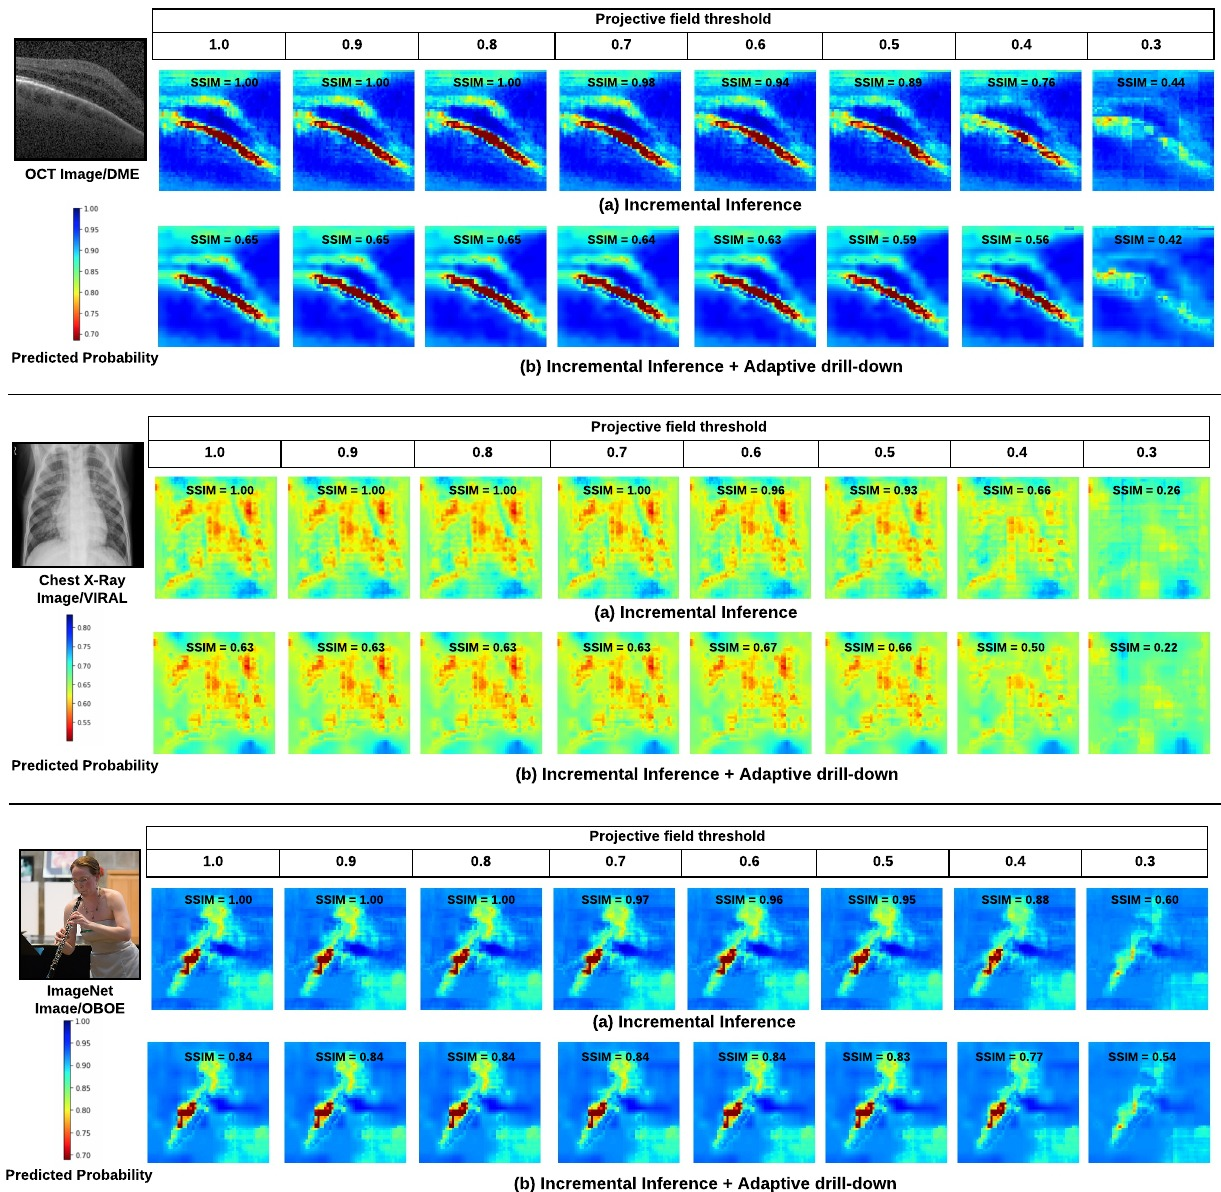
\includegraphics[width=\textwidth]{images/visual_examples}
\caption{Occlusion heat maps for sample images (CNN model = VGG16, occlusion patch size = 16, patch color = black, occlusion patch stride $(S~or~S_2)$ = 4. For \textit{OCT} $r_{drill\_down}=0.1$ and target \texttt{speedup}=5. For \textit{Chest X-Ray} $r_{drill\_down}=0.4$ and target \texttt{speedup}=2. For \textit{ImageNet} $r_{drill\_down}=0.25$ and target \texttt{speedup}=3).}
\label{fig:visual_examples}
\end{figure*}